%!TEX root = thesis.tex

\chapter{Results and Evaluation}
\label{chapter:Results and Evaluation}

This chapter will cover the subsystems and steps taken that were needed to achieve the testing environment described in Chapter~\ref{chapter:Proposed architecture}. This chapter will first discuss the arrangements related to the hardware of the framework and then software related arrangements will be presented and described. After presenting the built framework, achieved results will be discussed and finally the test environment presented in this Thesis will be evaluated.

\section{Hardware Arrangements}
\label{section:Hardware arrangements}

AAT environment presented in this master's thesis consists of several different hardware components. Environment had to be a smooth combination of manipulation and computing hardware and hardware architecture is thought to be modular in a sense that every component has a specific functionality. This allows easy maintenance and upgrade of each subsystem.

As stated in Chapter~\ref{chapter:Proposed architecture}, one of the requirements for this AAT environment was affordable price. For this reason hardware decisions have been made taking quality-price ratio into consideration and hobby-grade electronics were used widely through out the environment. 3D printing was also utilized as a manufacturing technique of custom made components for its relatively low manufacturing price and relatively acceptable quality of outputted plastic parts.

Main components of the AAT environment are the robot that handles the manipulation of the payment terminals, Raspberry Pi 2 Model B single-board computer which was used as a main computer of the environment, two Arduino Uno boards for more specific control needs of certain components, camera for machine vision and 3D printed payment card feeders for the payment terminals. These subsystems and components are described in following subsections.

\subsection{The Robot}
\label{subsection:Robot}

As suggested in Section \ref{subsection:The Robot proposal}, ShapeOko 2 open-source 3-axis CNC milling machine was used as robot manipulating the payment terminals. ShapeOko was built according to the instructions found from the homepage of the project (\emph{\cite{shapeoko}}). Construction was altered only regarding to the tool that was used as the spindle motor was substituted by 3D printed pushing tool.

ShapeOko 2 has a working area of about 300 mm x 300 mm x 60 mm and this means that it can accommodate up to three payment terminals at same time to the working area. This allows parallel test case execution i.e. test cases can be run at the same time with different terminals. Arrangement of the devices was implemented by dividing the work area into three sections. Each payment terminal was attached to a standard sized MDF-plate and each section of the working are can accommodate one of these MDF-plates. Holes were drilled in to the working area and nuts were inserted in to these holes at the back of the work bench. MDF-plates attach to these holes with screws enabling easy installation and removal of plates with different models of payment terminals. MDF-plates can be observed in Figure \ref{fig:card_feeder_2}.

\begin{figure}[ht]
  \begin{center}
    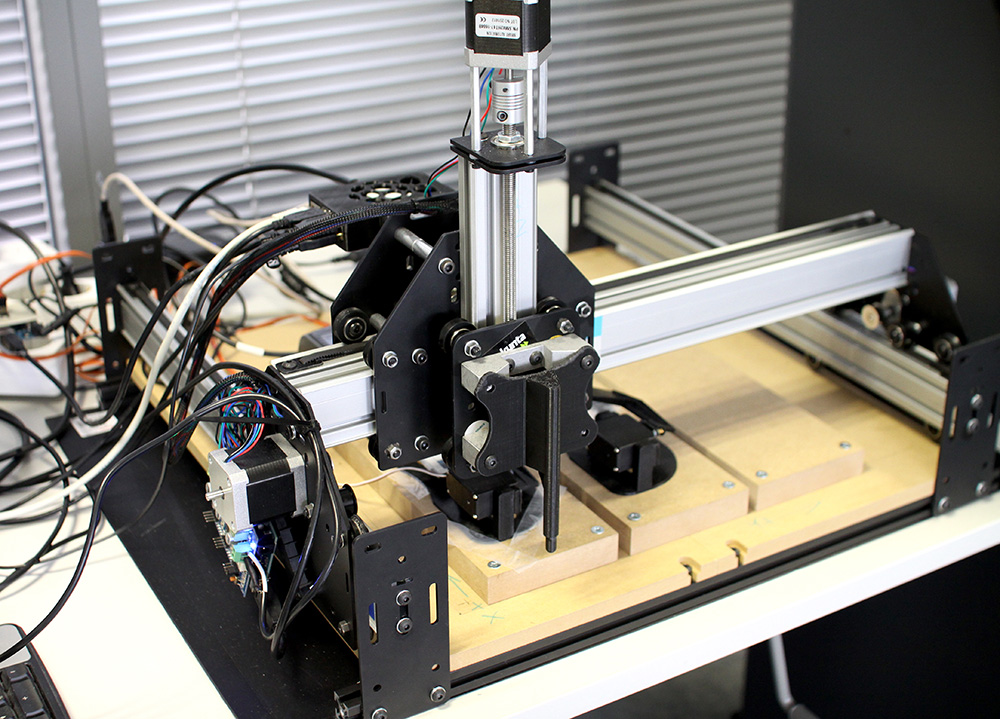
\includegraphics[width=10cm]{images/robot.jpg}
    \caption{Robot in its production state.}
    \label{fig:robot_final}
  \end{center}
\end{figure}
\FloatBarrier

Each axis of the robot is controlled by stepper motors. Use of stepper motors instead of servo motors offers affordable way of controlling each axis in a relatively fast and reliable manner. X- and Z- axises are both manipulated using one stepper motor on each axle and bigger Y-axis is manipulated using two parallel stepper motors. Manipulation of payment terminal buttons stresses the machine much less than actual milling of materials that the machine is designed for and this allows faster movement of the machine that would be possible when executing actual milling job.

The robot was controlled using G-code that was sent from the main computer to an Arduino Uno attached to the robot. Arduino Uno and the main computer were connected via USB connection. More detailed description of the electronics can be found from Section \ref{subsection:Computing hardware}.

Section \ref{subsection:The Robot proposal} suggested equipping the robot with a pushing tool and this was implemented to the final solution by 3D printing the tool from PLA plastic. Tool consisted of two parts: cylindrical beam and a stem inside of it. Stem slides inside the beam and the two parts are segregated with a spring. Spring provides the needed attenuation in order to forgive slight misalignments and too long trajectories when pushing the buttons of the payment terminals. Pushing tool can be observed in Figure \ref{fig:pushing_tool} and Figure \ref{fig:robot_final}.

\begin{figure}[ht]
  \begin{center}
    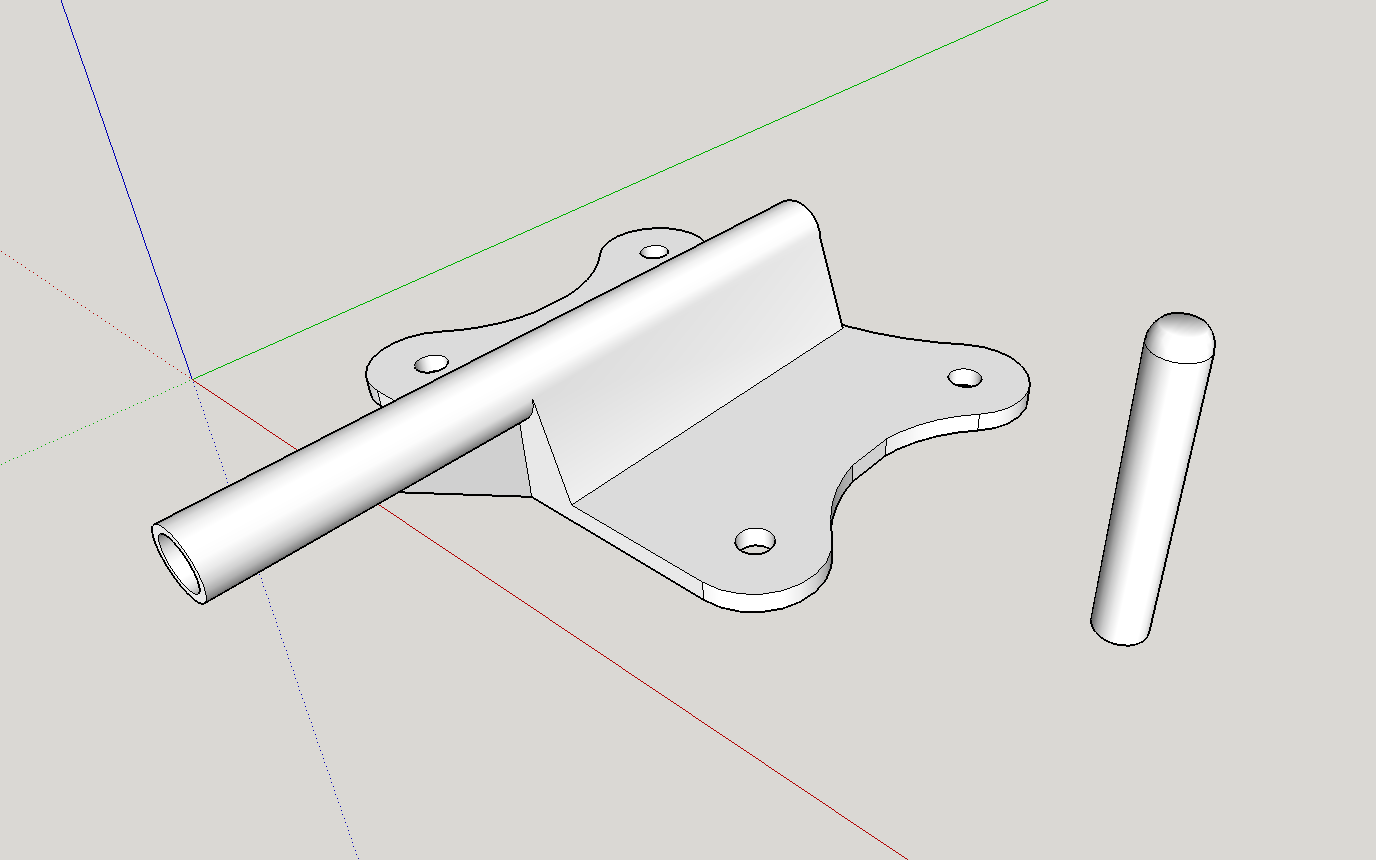
\includegraphics[width=10cm]{images/pushing_tool.png}
    \caption{CAD design of the pushing tool. Metal spring is inserted inside to the cylinder and the stem on the right side of the image slides to the cylinder.}
    \label{fig:pushing_tool}
  \end{center}
\end{figure}
\FloatBarrier

\subsection{Computing Hardware}
\label{subsection:Computing hardware}

Raspberry Pi 2 Model B single-board computer is used as a main computer of the AAT environment. Raspberry Pi provides optimal computing power compared to it's price and has big community of users and developers world wide. 3D printed enclosure was manufactured to protect the computer board and it was attached to the moving Z-axis assembly of the robot.

In addition to the Raspberry Pi 2, the robot also has two Arduino Uno boards for handling some specific functionalities of the AAT environment. One Arduino Uno is interpreting the G-code commands sent from the Raspberry Pi and it is connected to the stepper motors of the robot through a stepper motor driver shield (\emph{\cite{grbl_shield}}).

Second Arduino Uno is handling the servo motor control of the card feeders. It is connected to the Raspberry Pi via USB connection and control commands to Arduino Uno are sent using serial communication. Arduino Uno board provides PWM signal to the servo motors and can accommodate three card feeders at the same time. Self-made circuit board was fabricated and attached on top of the Arduino Uno board in order to make connecting the servo motor cables easy.

Connection diagram and main electronic components are visualized in Figure \ref{fig:electronics}.

\begin{figure}[ht]
  \begin{center}
    \includegraphics[width=10cm]{images/electronics.png}
    \caption{Main electronic components and connection diagram of the robot. Note that Y-axis is manipulated using two stepper motors.}
    \label{fig:electronics}
  \end{center}
\end{figure}
\FloatBarrier

\subsection{Camera Arrangements}
\label{subsection:Camera Arrangements}

As suggested in Section \ref{subsection:computer vision hardware}, Raspberry Pi's own camera module was used for machine vision hardware. Camera was attached to the bottom of the Raspberry Pi's enclosure and the enclosure was attached to the Z-axis assembly of the robot to the opposite side where the pushing tool is. Camera can be moved within the X- and Y-axis. Z-axis movement of the camera isn't possible. Depth of focus of the camera provides clear image of the screen even when the distance between the lens and the screen differs slightly between different payment terminal models. Camera attachment can be seen in Figure \ref{fig:camera}.

\begin{figure}[ht]
  \begin{center}
    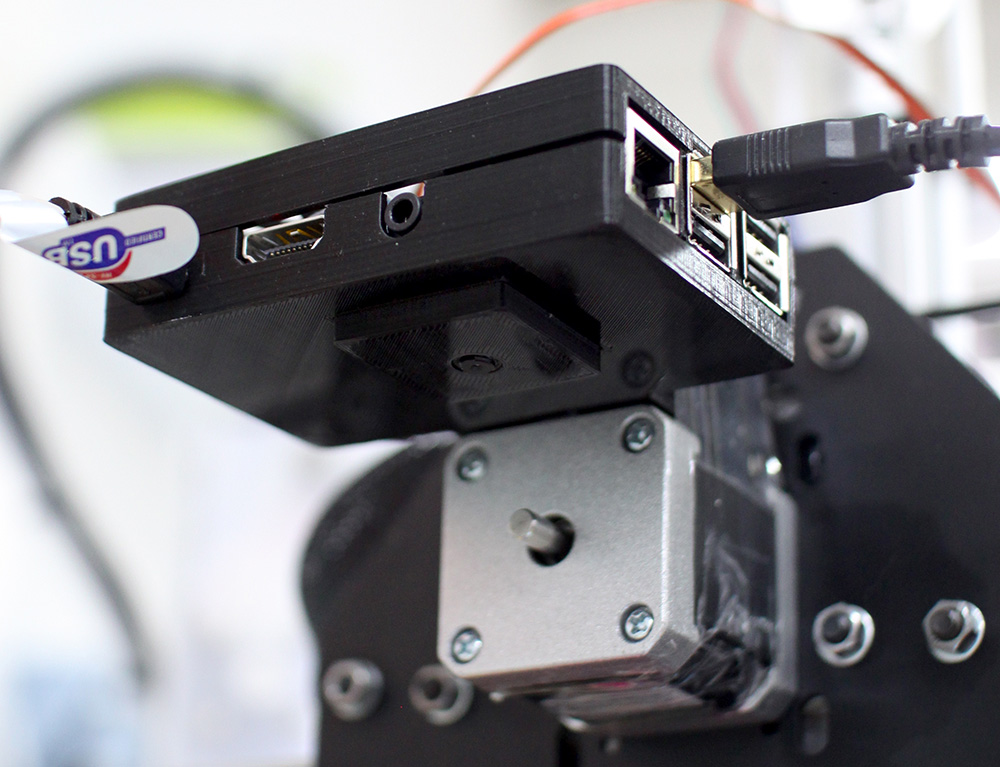
\includegraphics[width=10cm]{images/camera.jpg}
    \caption{Camera is attached to the bottom of the Raspberry Pi's enclosure. Image also shows the attachment of the Raspberry Pi enclosure to the Z-axis assembly of the robot.}
    \label{fig:camera}
  \end{center}
\end{figure}
\FloatBarrier


\subsection{Card Feeder Arrangements}
\label{subsection:Card feeder arrangements}

As suggested in Section \ref{subsection:Card feeder}, card feeder structures were 3D printed using PLA plastic. Finalized card feeders consisted of bottom plate, payment card holder and servo motor. Servo motor attaches directly to the bottom plate and card holder attaches to the arm of the servo motor.

Simplistic design can be used with different kinds of payment terminals which have the card slot at the bottom edge of the device. Flexibility provided by the plastic structure and the payment card itself allows the solution to be compatible with most of the payment terminals of this type. Design of the card feeders is presented in Figure \ref{fig:card_feeder}. Figure \ref{fig:card_feeder_2} shows ready part installed to the environment presenting the servo installation and attachment of the card holder to the servo arm.

\begin{figure}[ht]
  \begin{center}
    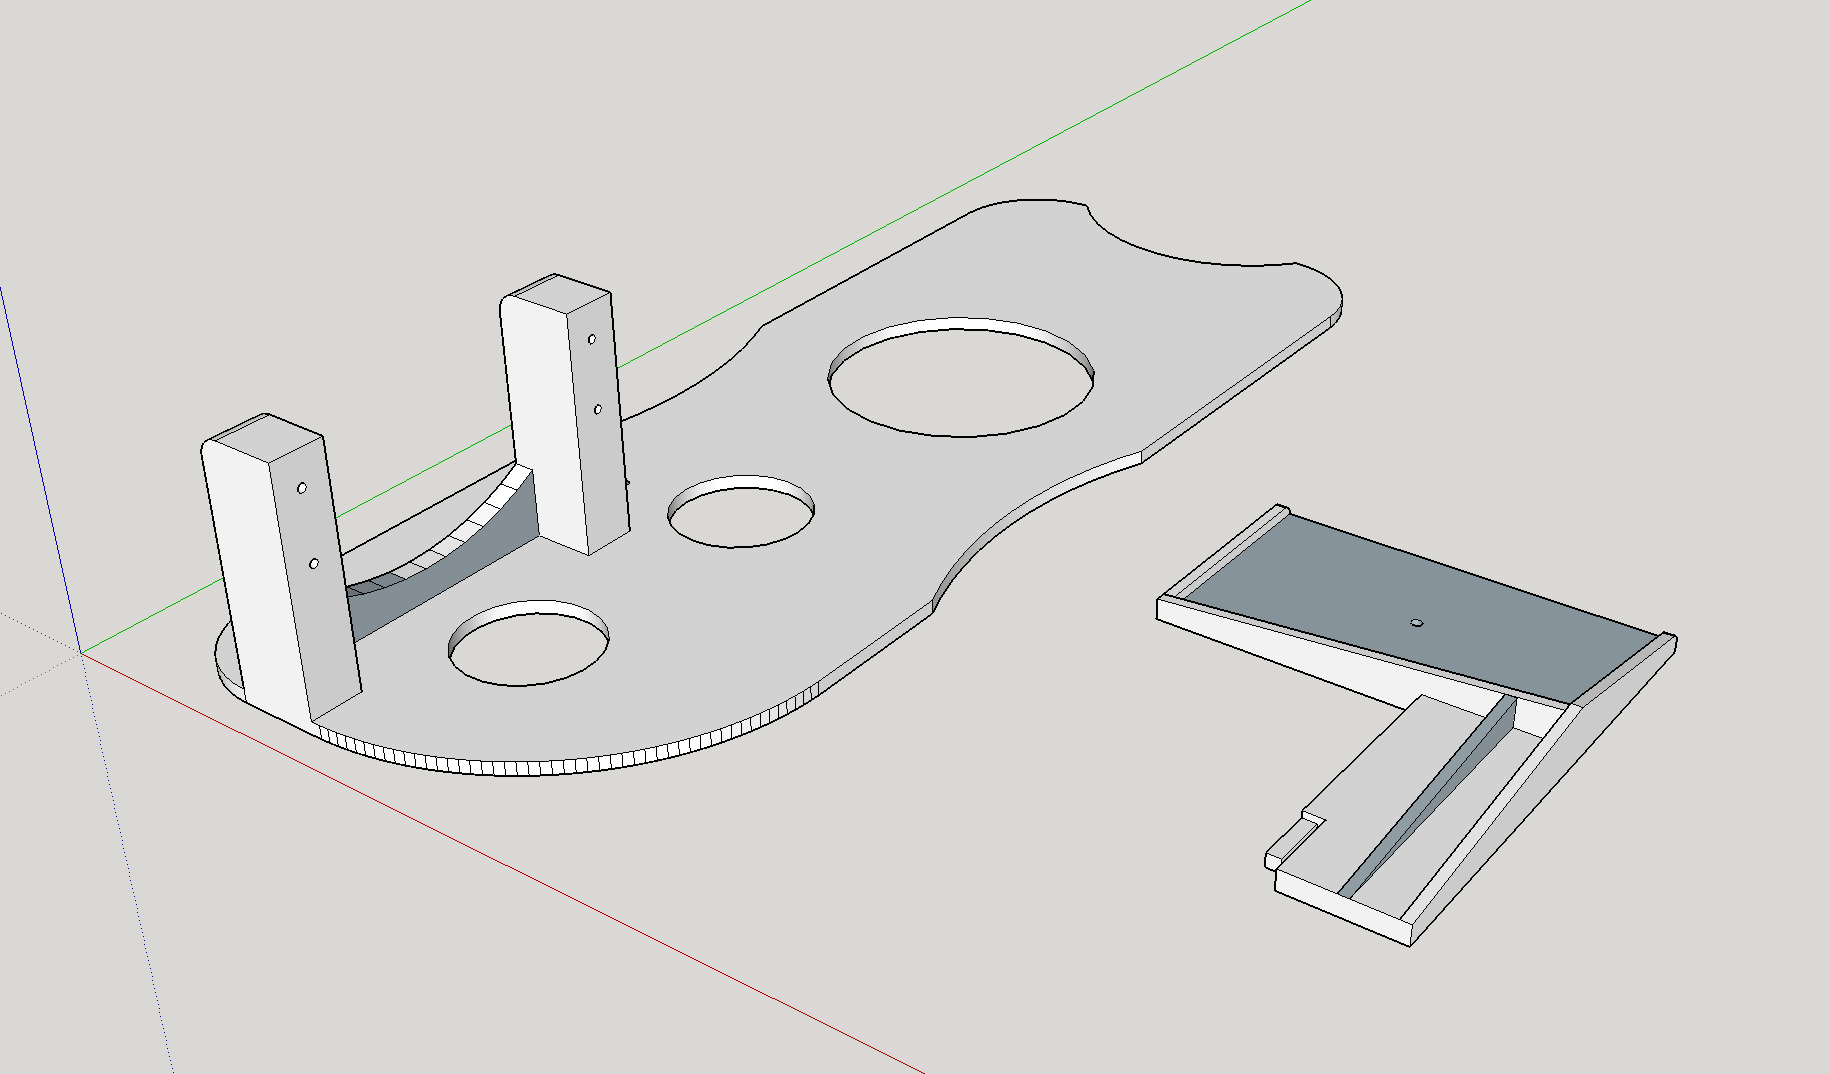
\includegraphics[width=8.4cm]{images/card_feeder.png}
    \caption{CAD design of the card feeder. Servo motor attaches to the bigger plate on the left and card holder on the right attaches to the arm of the servo motor. Card holder is designed to fit standard sized payment card.}
    \label{fig:card_feeder}
  \end{center}
\end{figure}

\begin{figure}[ht]
  \begin{center}
    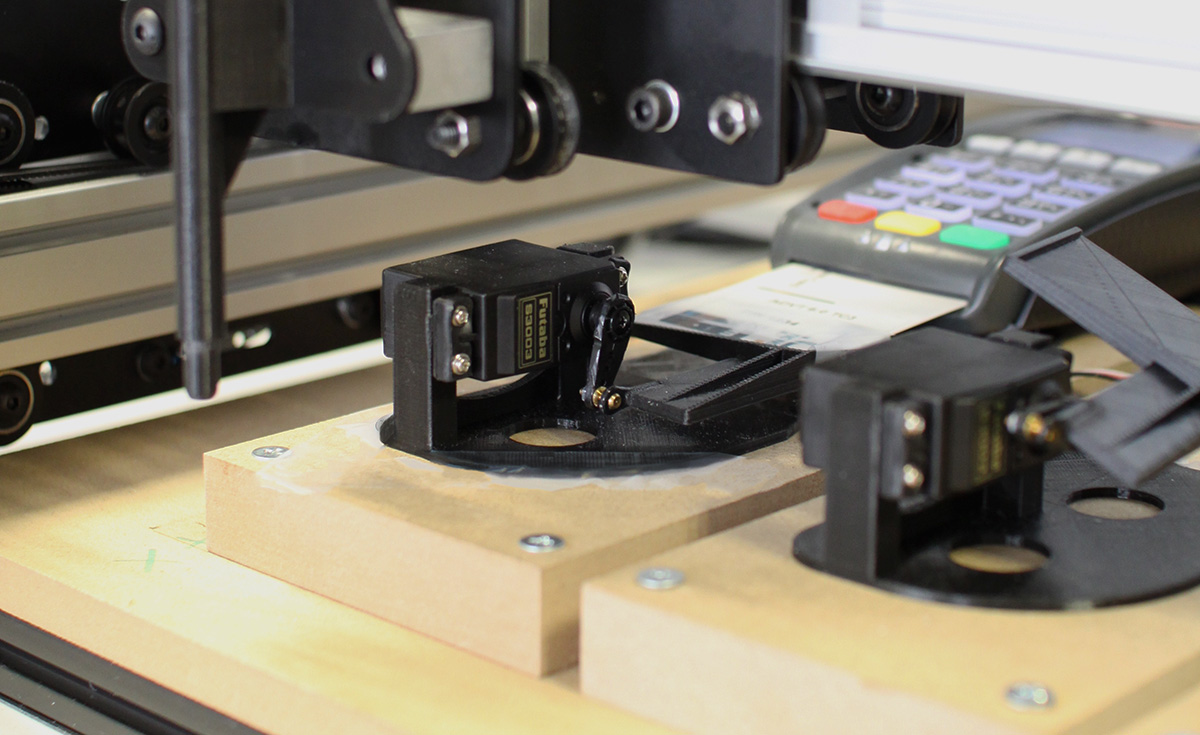
\includegraphics[width=8.4cm]{images/card_feeder_2.jpg}
    \caption{Card feeder installed to the environment. Image also presents the idea of MDF-plates described in Section \ref{subsection:Robot}.}
    \label{fig:card_feeder_2}
  \end{center}
\end{figure}
\FloatBarrier

\section{Software Arrangements}
\label{section:Software arrangements}

As proposed in Section \ref{section:software}, this chapter will describe decisions and arrangements regarding to the software point of view of the AAT environment. Proposal was followed rather loyally though some additional arrangements had to be implemented to the environment in order to increase usability and effectiveness.

Modular architecture was implemented also to the software level similar to the hardware level. Implementation only included open source or self made software components from the operating system to individual software libraries used in the AAT environment.

This section describes the individual software components of the AAT environment and their usage and function in the whole system. System configuration, test framework and libraries and the final test suite syntax will be presented.

\subsection{Software Architecture}
\label{subsection:Software architecture}

Suggested already in the Section \ref{section:software}, Raspbian Wheesy Debian-based operating system was used with the Rasbperry Pi 2 Model B single-board computer. Operating system was used to run the test framework, test libraries and other software components and to handle the communication with different subsystems of the AAT environment.

Robot Framework was used as a test framework for its modularity, simplicity and versatility. RF was run on top of Python runtime environment and all test libraries were written using Python programming language (\emph{\cite{python}}). Python test libraries were implemented to handle the needed serial communication to the Arduino board on ShapeOko 2 and to the other Arduino board used for controlling the card feeder servo motors. Picamera Python library was used for providing the needed Python interface for communication with the Raspberry Pi camera module (\emph{\cite{picamera}}). Overall visualization of the software architecture can be observed in Figure \ref{fig:software_architecture}.

As different keyboard layouts have to be supported, configuration files for keyboard layouts were implemented. There are two types of configuration files: one for device locations in the working area of the robot and one for each keyboard layout. Configuration file for device locations defines the coordinates of "number one" -button and the height in respect of Z-axis where the transitions over the buttons are safe. This is Z-axis coordinate is used for transitions between pressings of buttons. 

Configuration file for each keyboard layout defines the button locations in respect to the "number one" -button. Z-axis coordinates defined in this file define the distance from the safe transition height to the full press of the button. Location of the screen of each device is also defined in these configuration files and it is used for driving the robot to the optimal place for capturing the image of the display of the device under test. 

By dividing the configuration files into different levels enables easy modification and adding of new device configurations. Desired configurations can be also changed easily at the test case level. Examples of these configuration files can be observed in Figure \ref{fig:conf1} and in Figure \ref{fig:conf2}.

\begin{figure}[ht]
  \begin{center}
    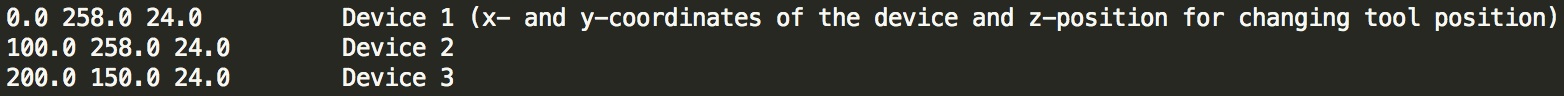
\includegraphics[width=\textwidth]{images/conf1.png}
    \caption{Configuration file for device locations in the working area of the robot.}
    \label{fig:conf1}
  \end{center}
\end{figure}
\FloatBarrier

\begin{figure}[ht]
  \begin{center}
    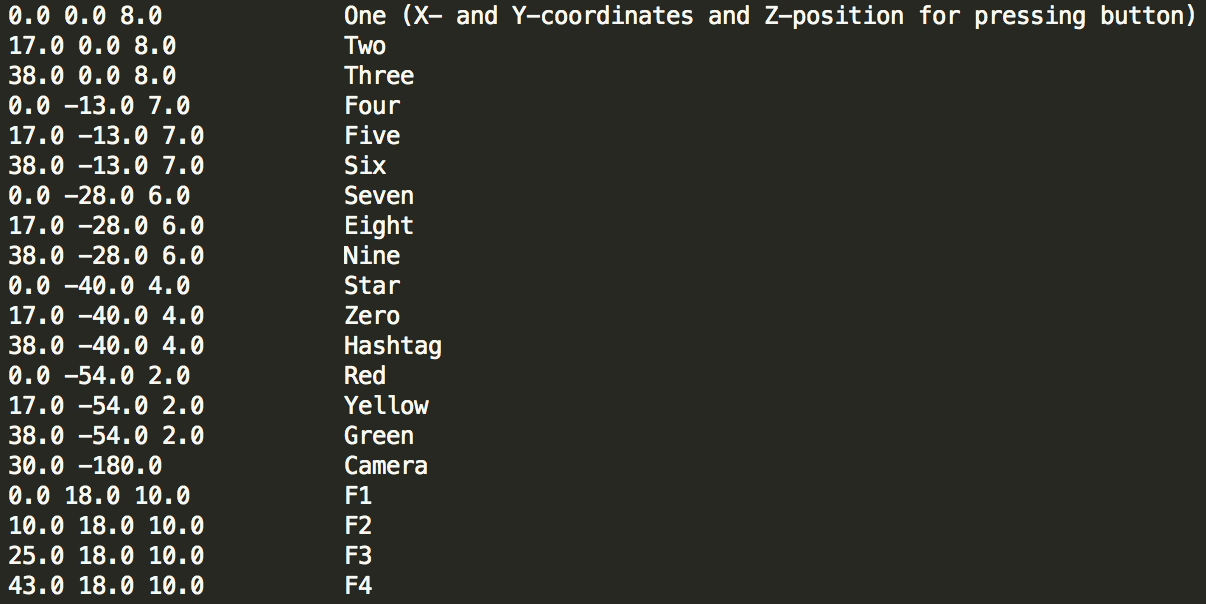
\includegraphics[width=11	cm]{images/conf2.png}
    \caption{Example of a configuration file of a device keyboard layout.}
    \label{fig:conf2}
  \end{center}
\end{figure}
\FloatBarrier

\begin{figure}[ht]
  \begin{center}
    \includegraphics[width=12cm]{images/software_architecture.png}
    \caption{Simplified visualization of the software architecture of the AAT environment.}
    \label{fig:software_architecture}
  \end{center}
\end{figure}
\FloatBarrier

\subsection{Robot Framework Test Framework}
\label{subsection:Robot Framework and libraries}

As proposed in Section \ref{subsection:test framework}, Robot Framework was used as a test framework for AAT environment presented in this master's thesis. RF was equipped with several different test libraries to achieve the desired functionality of the AAT environment.

RF is a generic keyword driven test framework and this means that the keywords used for different test steps can be defined in desired level of abstraction, lowest being that one keyword would handle only one library method and highest being that one keyword would be responsible of whole test case. This allows high versatility but also makes the developer responsible of writing test cases according to commonly accepted best practices. Test cases developed in the scope of this master's thesis were developed to be as human readable as possible and to mimic the mindset of human when dividing the test cases into steps. This naturally depends of the person that is thinking the test steps but it was attempted to make the devision between each test steps as clear as possible.

Test cases and steps were also divided into different keywords in a sense of reusability. According to \emph{\cite{clean-code}} any code written should be as readable and understandable as possible and these directions were used as guidelines when the test cases were implemented. \emph{\cite{clean-code}} also advices that code should be written in highly modular manner and this was followed when the keywords were combined in different abstraction levels.

Keywords used in test cases were defined in three different levels: test library keywords, shared keywords and test suite specific keywords. Test library keywords are the most low level keywords and implement the functionality between RF and SUT using different interfaces. These were written using Python language. 

AAT environment also introduced a resource file for combining the keywords that were shared with different test suites. Abstraction level of keywords found from this file can be qualified as middle or high level. Resource file is also used for defining common test libraries between test suites and common set-up and tear-down commands of test cases and suites. Resource file is imported to each test suite file. Example of partial resource file can be seen in Figure \ref{fig:resource}

Based on the work done in this master's thesis, open source RF library was published (\emph{\cite{cnc-library}}). This library can be used for easy controlling of devices that use serial communication as a communication protocol and are controlled using G-code commands. library is intended for use in similar circumstances described in this master's thesis but can also be used as general G-code control library for Robot Framework.

\begin{figure}[ht]
  \begin{center}
    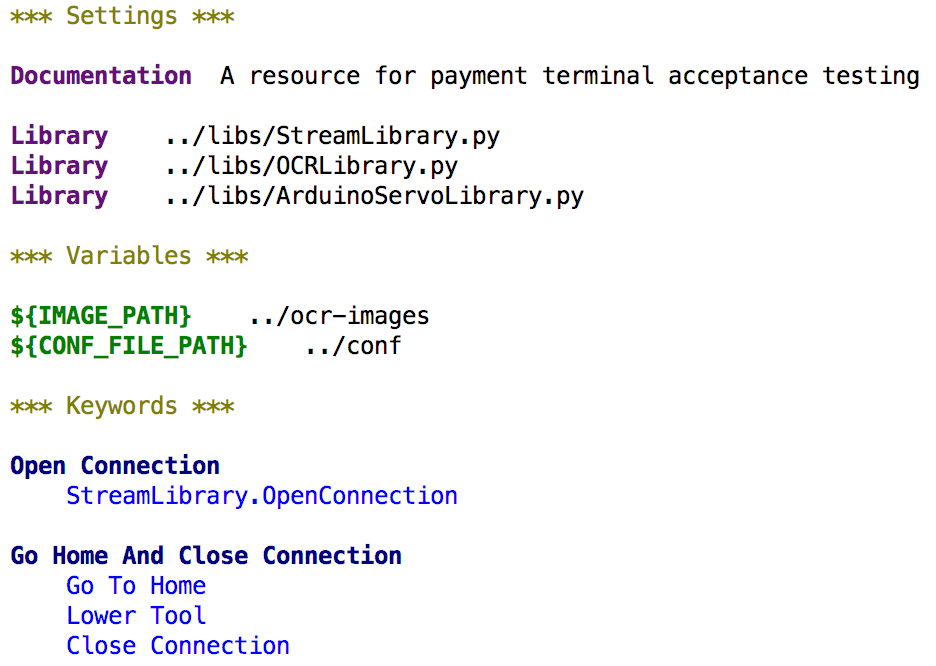
\includegraphics[width=12cm]{images/resource.png}
    \caption{An example of a partial resource file for Robot Framework tests.}
    \label{fig:resource}
  \end{center}
\end{figure}
\FloatBarrier

\subsection{Robot Control and Card Feeder Libraries}
\label{subsection:libraries}

For sending the control commands to the ShapeOko 2 robot with Robot Framework, robot control library was implemented using Python language. Control commands for the robot robot are given using G-code commands and those are being sent using serial communication protocol. Library defines keywords that can be used withing the keyword definitions and test cases of the RF acceptance tests.

Desired G-code commands are produces in respect to the configuration files described in Section \ref{subsection:Software architecture}. Library reads the coordinates of the devices and different buttons and by combining these forms the needed G-code command to drive the robot into particular location. Library has \emph{go\_to()} -method which takes the button name as parameter to drive the robot into desired position. \emph{press\_button()} -method is used to press the button when to robot is reached the desired position on top of the button.

Library also has methods for setting the home position which is used in the initialization of the library after it has been imported into RF test. Library also implements methods for going into home position, going to the right position for image capture in respect of the device under test and individual methods for lovering and raising the pushing tool of the robot. These can be used as a keywords within the test cases.

For controlling the card feeder another test library was also implemented using Python language. Control command for card feeder Arduino board are being sent using serial communication and library takes care of this interaction between the RF and the Arduino board. Card feeder library only implements \emph{update()} -method that takes the angle and the card feeder number as parameters. This method sends the control command to the Arduino board of the card feeders and can be used as a keyword within the RF keywords or test cases.

\subsection{Card Feeder Software}
\label{subsection:card feeder software}

For controlling the servo motors of the card feeders with Arduino board, an Arduino program was developed. As described in previous section, the control commands are sent to the Arduino using serial communication. Messages read by Arduino consists of two parts: card feeder number and desired angle of the servo. After receiving the message, Arduino program interprets the device number and angle from it and uses switch-case code structure to control the appropriate card feeder. 

Servo motors of the card feeders are controlled using PWM control signals. Arduino program can drive the servo motors to every angle that the servo motor is capable of moving and the angles of inserting the card and removing the card can be defined in the test case level.

\subsection{Computer Vision Library}
\label{subsection:Computer vision library}

As proposed in Section \ref{subsection:test libraries}, computer vision library was implemented for extracting the optical features on the display to format that can be interpreted programmatically. The main task of the computer vision library is to interpret the text displayed in the screen of the payment terminal.

Computer vision library was implemented using Python language and Tesseract optical character recognition (OCR) engine is used to extract the found characters to textual format. Image captured by the Raspberry Pi camera module is slightly manipulated in order to make the text extraction more efficient and reliable. Image manipulations are made using OpenCV Python library (\emph{\cite{opencv}}). Image is first being slightly blurred using Gaussian blur filter in order to reduce the amount of disturbance caused by pixel edges of the display. Color space of the image is then converted to gray-scale. Finally, the gray-scale image is converted into binary BW image by comparing the pixel value to certain threshold value. Threshold value is adjusted according to the screen brightness and lightning conditions of the space where the robot is situated. These image manipulations produce an image where text in the display is clearly distinguishable from the other features providing good foundation for the character recognition.

Tesseract OCR engine can basically extract any kind of common characters from the image and this can sometimes cause unwanted noise as small dirt particles and disturbances in the image can be interpreted to some exotic special character. In order to make the task of OCR engine easier in addition to the binary BW image, possible characters are white-listed. Final list of possible characters that are accepted by the OCR engine is: "ABCDEFGHIJKLMNOPQRSTUVWXYZabcdefghijklmnopqrstuvwxyz0123456789,\euro". This also helps the OCR engine to distinguish right characters from possible similar looking foreign-language counterparts.

Computer vision library outputs all found textual features from the source image and validation of right content is being done using Robot Framework. 

\subsection{Test Syntax}
\label{subsection:Test syntax}

Robot Framework files are divided into different parts that all have specific functionality and purpose. This helps to observe the different configurations and used keywords within the test suite in order to gain comprehension of the functionality of the particular file. As mentioned earlier, the project structure is divided into shared resource file and individual test suite files. Same syntax applies to both kinds of files, only the scope of the definitions changes according to the type of the file. Resource file is divided into three sections: settings, variables and keywords. Test suite files are divided into four sections: settings, variables, test cases and keywords.

Settings section of the file define all the needed settings for executing the test cases. This includes all resource and library imports and test setup and teardown definitions. In this project all the library imports are done within the resource file and the resource file is imported to the test suites in the settings section of the test suite files. Test teaedowns are also defined at test suite level.

Variables section defines all the used variables within the test cases. Variables section of the resource file are used for defining used directory paths for e.g. location of the image directory used by the computer vision and location of the configuration files of the device location configuration file and configuration files of different keyboard layouts of the payment terminals. Variables are defined using \emph{\$\{variable\}} annotation.

Test cases section of the test suite files are used for defining all the test cases within the test suite and test steps of the test cases. Test cases are defined by naming them in the firs line and then defining the test steps by indenting the names of the used keywords with at least two space characters under the name of the test case.
    
Keywords are defined in the same way as test cases. Each keyword definition begins with the name of the keyword followed by indented names of used lower level keywords or library methods. Keywords can be built modularly into different layers by using lower lever keywords in higher level keyword definitions.

Example test case can be seen in Figure \ref{fig:invalid_pin_test} as proposed test case syntax was followed.

\subsection{Test Results}
\label{subsection:Test result syntax}

For the testing to be actually useful and informative, clear test reports and error descriptions has to be generated. Robot Framework is useful for this purpose as it automatically generates two types of clear and easily understandable test result files after executing the test suite under examination. These files are outputted in \emph{.html} format making it able examine the reports interactively using web browser.

\emph{report.html} file can be user to review the overall status of executed test suites and cases. This report gives overall view to the testing project and different outcomes of the tests are marked in bright colors green representing passed test and red representing failed test. Example of passed test report file can be seen in Figure \ref{fig:passed report} and example of failed test report can be seen in Figure \ref{fig:passed report}.

\emph{log.html} file contains more detailed representation of the test cases. Each test step is shown here and the internal keywords and library methods used by the keyword are layered under each test step. If test step fails during the test execution, the stack trace of that particular command is added to the log file and can be easily observed. Example of log file can be seen in Appendix \ref{chapter:first-appendix}.

Robot Frameworks also allows setting up threshold limits for test suites that are used to determine whether the test suite is passed or failed. For example, the threshold can be set to 90 \% and if over 90 \% of test cases within the test suite are passed, the test suite is being considered passed. Test cases can also be marked as critical meaning that if those particular test cases fail, the test suite is never considered as passed.

\begin{figure}[ht]
  \begin{center}
    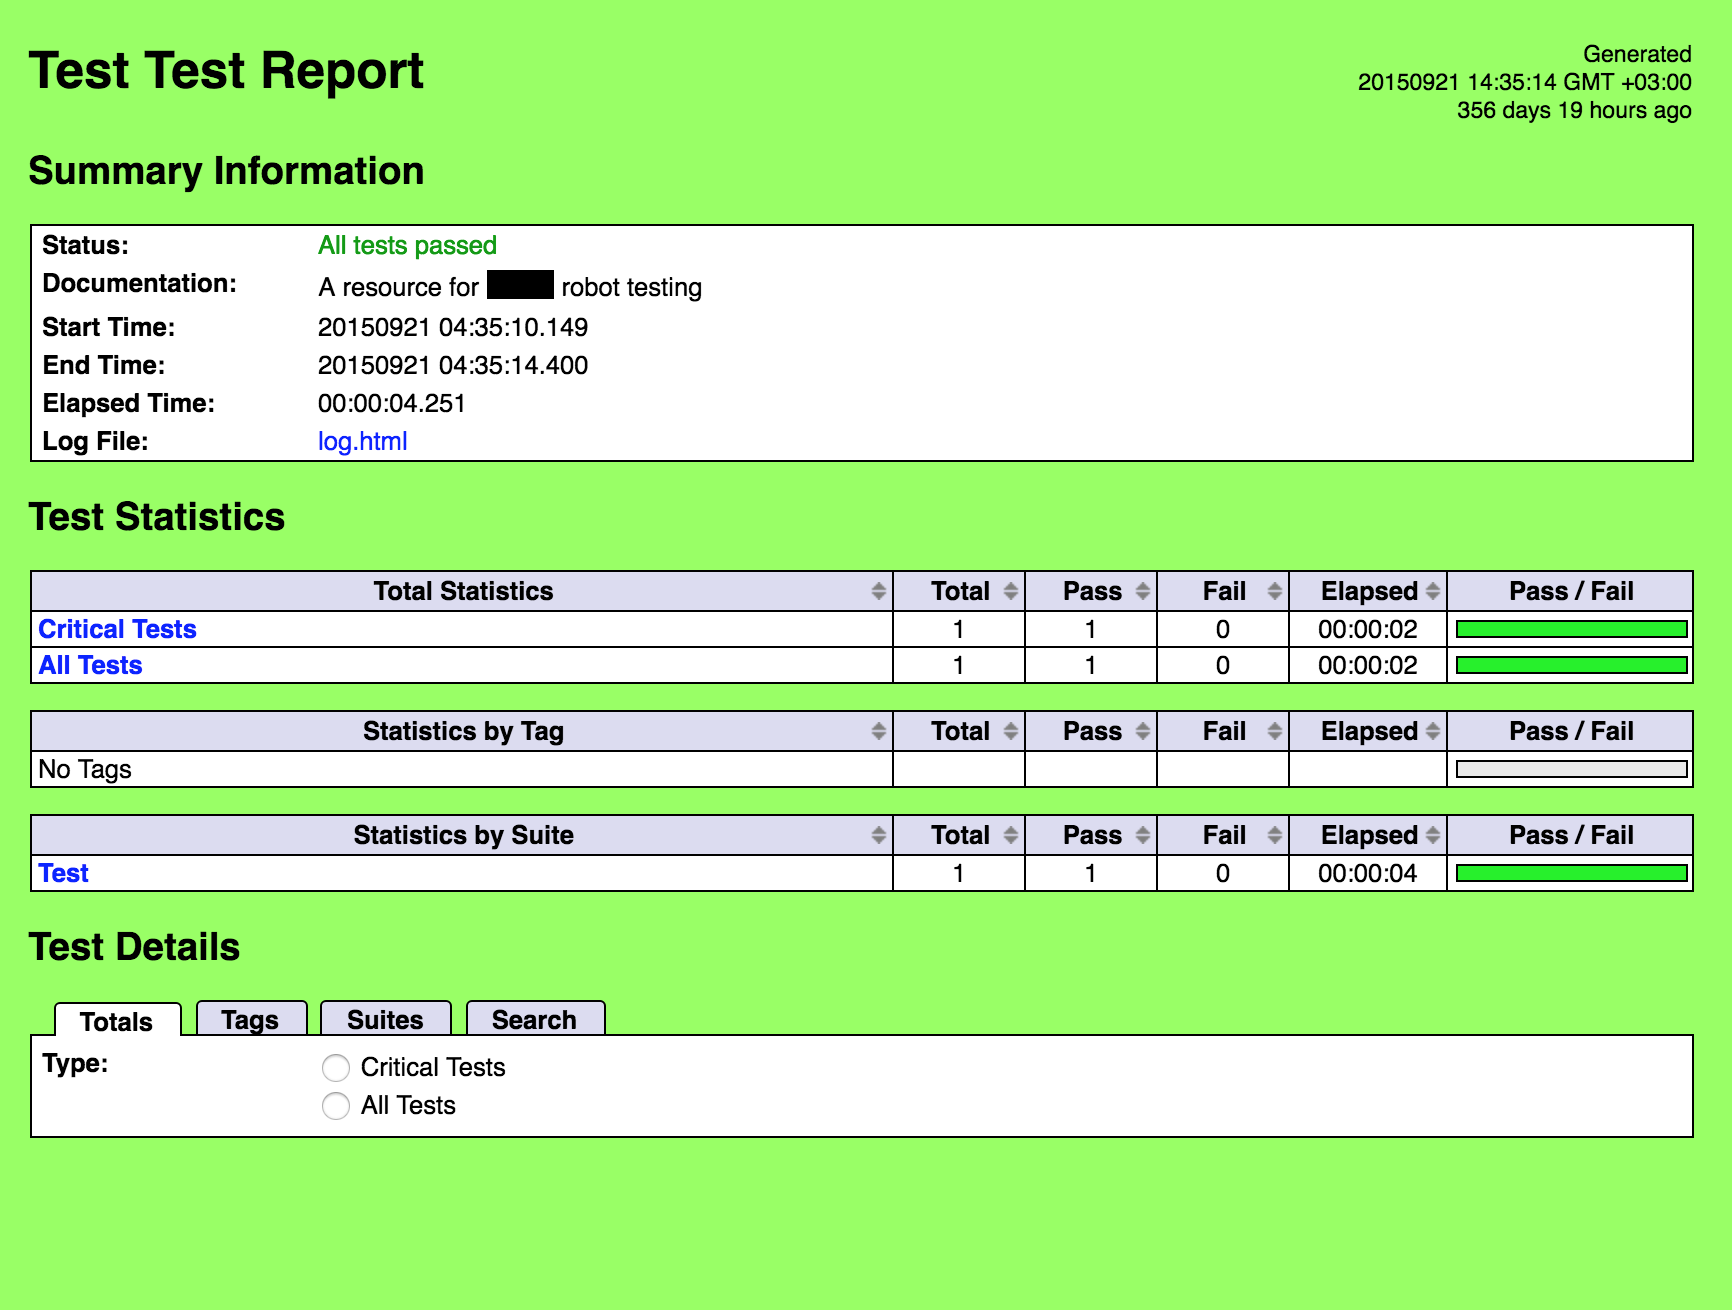
\includegraphics[width=.8\textwidth]{images/passed_report.png}
    \caption{Report of passed tests.}
    \label{fig:passed report}
  \end{center}
\end{figure}
\FloatBarrier

\begin{figure}[ht]
  \begin{center}
    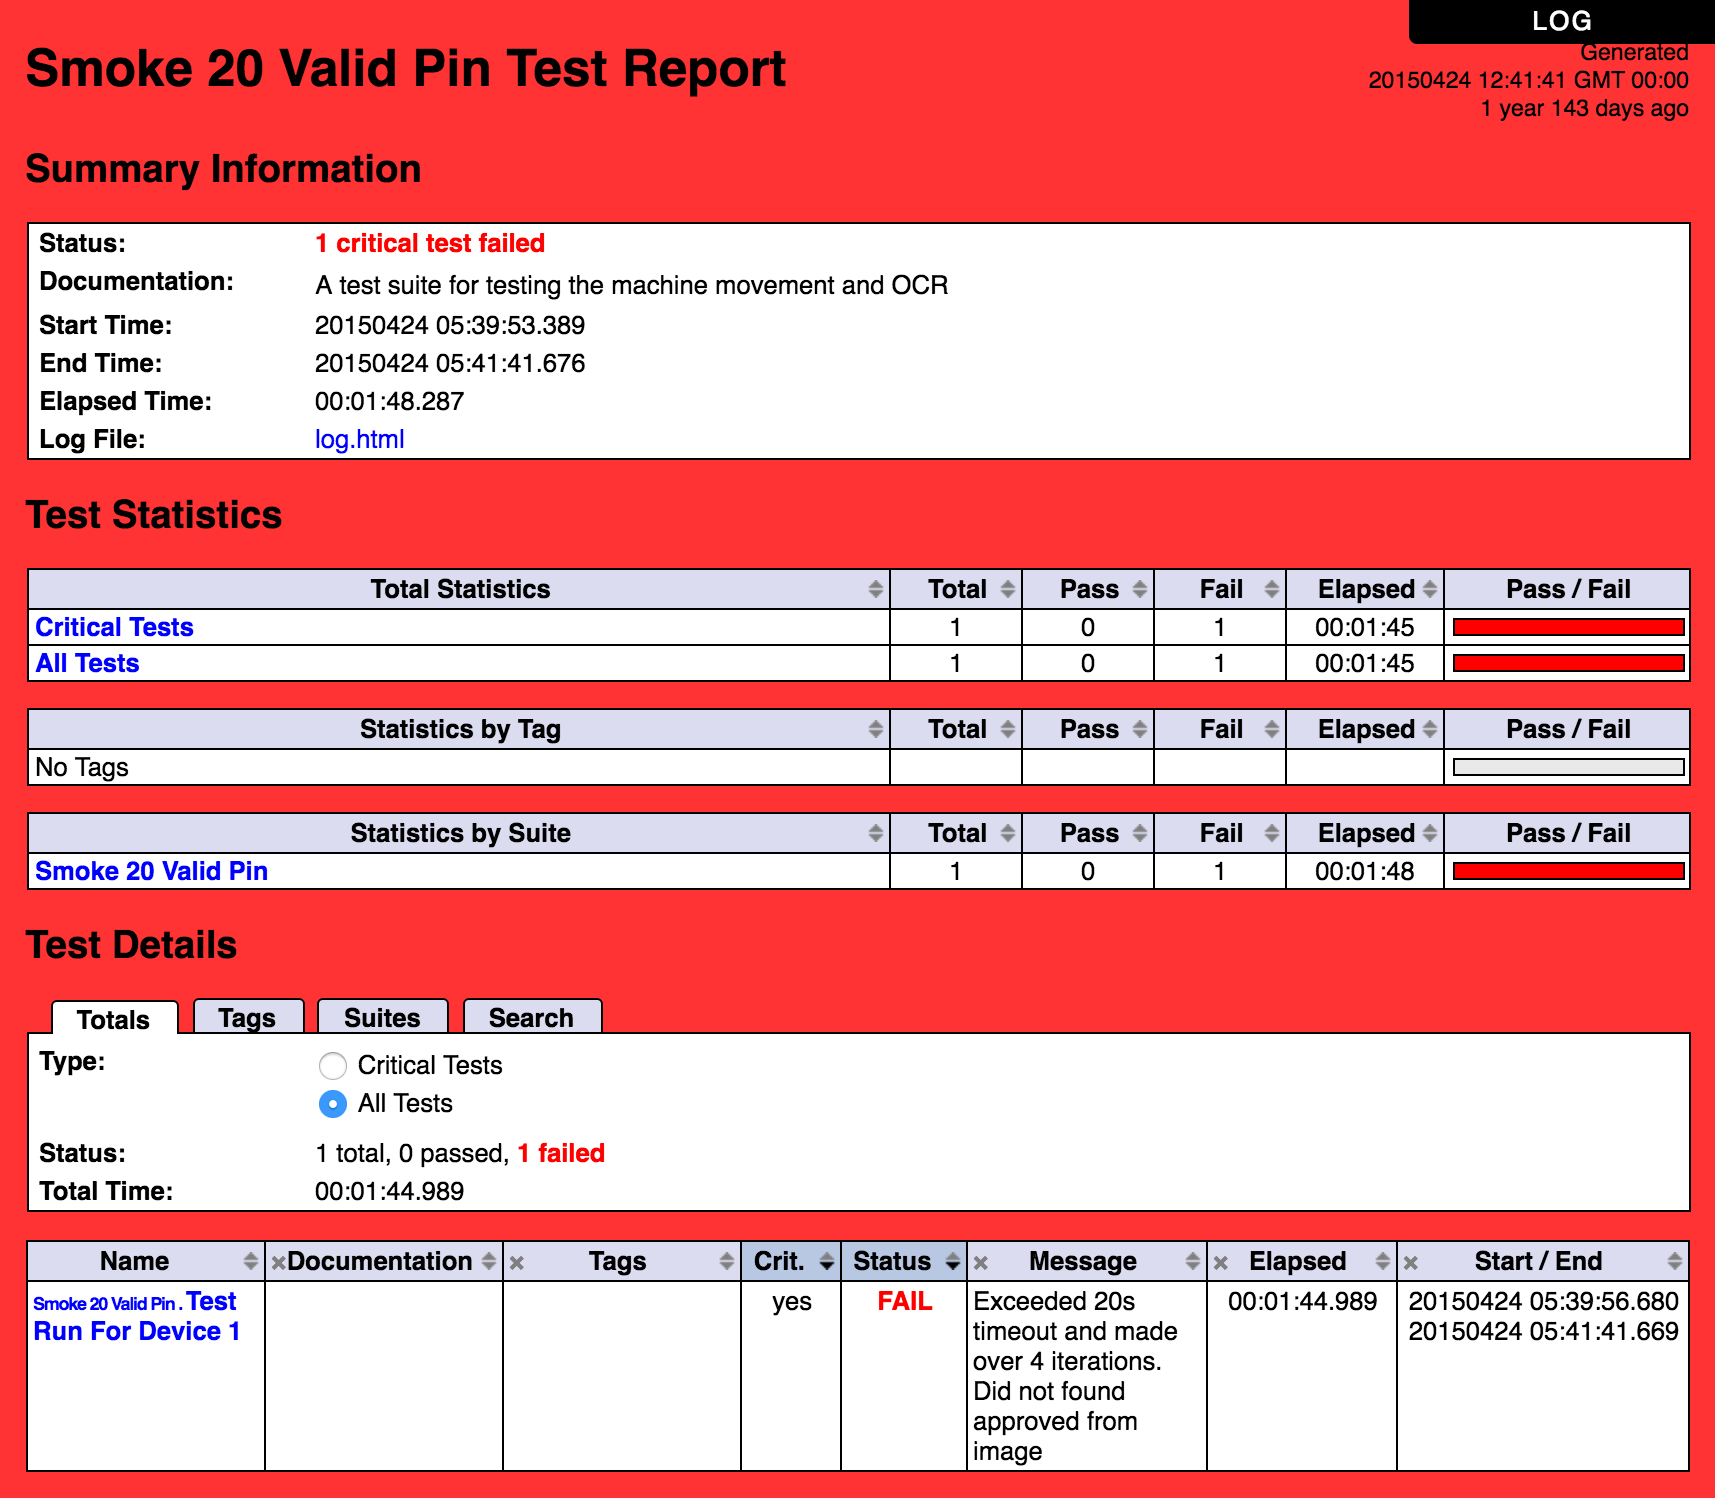
\includegraphics[width=.8\textwidth]{images/failed_report.png}
    \caption{Report of failed tests.}
    \label{fig:failed report}
  \end{center}
\end{figure}
\FloatBarrier